\documentclass[a4paper,12pt]{report}
\usepackage[utf8]{inputenc}
\usepackage[T1]{fontenc}
\usepackage[english]{babel}
\usepackage{lmodern}
\usepackage{multirow}
\usepackage{chngpage}

%Figure progressive enumeration
\usepackage{chngcntr}
\counterwithin{figure}{chapter}
\counterwithin{table}{chapter}

%package used to enumerate figures
\usepackage[labelfont=bf]{caption}

%hyperref for interactive PDF index
\usepackage[bookmarks, colorlinks, breaklinks]{hyperref}
\hypersetup{linkcolor=black, citecolor=black, filecolor=black, urlcolor=black}

%Package required to use special symbols
\usepackage{amsmath, amssymb}

%Package required to use figures
\usepackage{graphicx}
%Include the bibliography in the table of contents
\usepackage{tocbibind}

%Package used to insert figures at the specified position
\usepackage{float}

%Our chapters must be called sections
\addto\captionsenglish{\renewcommand{\chaptername}{Section}}

\begin{document}

%Code for title page
\begin{titlepage}
\centering
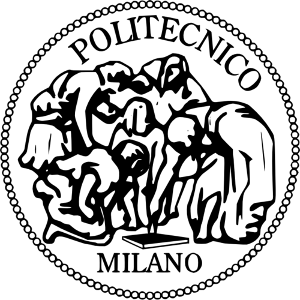
\includegraphics[width=0.20\textwidth]{./pictures/logo_poli}\par
	\vspace{1.5cm}
	{\Large {PowerEnJoy \\ 
		Software Engineering II} \par}
	\vspace{1.5cm}
	{\LARGE \textbf{Project Plan Document} \par}
	\vspace{1.5cm}
	{\Large\itshape Giovanni Scotti, Marco Trabucchi\par}
	\vspace{2cm}
	\vfill
	% Bottom of the page
	{\large Document version: 1\par}
	{\large \today \par}
\end{titlepage}

%Make the table of contents
\tableofcontents

\chapter{Introduction}
\section{Purpose and Scope}
The purpose of this document is to provide a reasonable estimate of the complexity of the \textit{PowerEnJoy} project in terms of the development team effort.

In the first section of the document, two complementary estimation models, \textit{Function Point Analysis (FPA)} and \textit{COCOMO II}, are going to be used in order to support the estimation process; the result will be an estimate of the number of lines of source code (SLOC) to be written and the average effort required for the development process itself.

In the second section, the organizational structure of the project plan will be laid down; here will be defined a possible schedule to cover all activities within the deadline and with a proper redistribution of tasks among the team members.

The last section of the document contains an analysis of all kinds of risks that the project could be facing throughout its life-cycle, from the development phase to the deployment phase, up to the maintenance and support phase. Here are also defined the safety measures, both reactive and pre-emptive, to face the eventual occurrence of the risks mentioned above.

\section{Definitions, Acronyms and Abbreviations}
\begin{description}
\item[COCOMO:] COnstructive COst MOdel
\item[DD:] Design Document
\item[EI:] External Inputs
\item[EIF:] External Interface Files
\item[EO:] External Outputs
\item[EQ:] External Inquiries
\item[FP:] Function Point
\item[FPA:] Function Point Analysis
\item[ILF:] Internal Logic Files
\item[ITPD:] Integration Test Plan Document
\item[LDF:] Language-Dependent Factor
\item[RASD:] Requirements Analysis and Specification Document
\item[SLOC/KSLOC:] Source Lines Of Code / Kilo Source Lines Of Code
\end{description}

\section{Reference Documents}
The indications provided in this document are based on the ones stated in the previous deliverables for the project, the RASD document~\cite{rasd}, the DD document~\cite{dd} and the ITPD document~\cite{itpd}.

Moreover it is strictly based on the specifications concerning the RASD assignment~\cite{se-assignments} for the Software Engineering II project, part of the course held by professors Luca Mottola and Elisabetta Di Nitto at the Politecnico di Milano, A.Y. 2016/17.

To support the application of the COCOMO II model estimate, the COCOMO II Model Definition Manual~\cite{cocomo-manual} has been followed.

\chapter{Function Points Estimation}
This chapter is devoted to the Function Point Analysis for the \textit{PowerEnJoy} project, aimed at obtaining a reasonable estimate of the size of the project, which will be later used within the COCOMO II estimation model to compute an average effort factor for the development process.

\section{Function Points Analysis}
\subsection{Internal Logic Files (ILFs)}
Internal Logic Files are defined as follows~\cite{cocomo-manual}:
\begin{quotation}
\textit{"Internal Logic Files count each major logical group of user data or control information in the software system as a logical internal file type. They include each logical file (e.g., each logical group of data) that is generated, used, or maintained by the software system."}
\end{quotation}
\noindent
In practice, they can be identified as a homogeneous set of data used and managed by the application itself.

The identified ILFs for the application are:
\begin{description}
%info account, info pagamenti, info posizione, reservation history, alto numero istanze, molti attributi --> HIGH
\item[ILF1] \textbf{User data}: identifies and groups all data pieces about users: information about user accounts, lists of user payments, positional information, reservation histories. The Function Point complexity can be set to \textit{HIGH}, since user-related entities will be generated and used by the application in great number and the level of detail of said data pieces will be considerable: attributes for involved data structures will be many.
%info stato macchina, info posizione, numero istanze molto stabile e di qualche ord grand inferiore risp a utenti, numero considerevole di attributi ma non moltissimi --> LOW
\item[ILF2] \textbf{Car data}:	identifies and groups all data about the application-managed vehicles: car status and availability, positional information. The number of instances related to this data group will be much more contained in number when compared with those of the \textbf{User data} group, and will also include a smaller number of attributes; hence, the complexity level can be set to \textit{LOW}.
%info pagamento semplici, solo mantenuto, pochi attributi, numero istanze elevato --> LOW
\item[ILF3] \textbf{Payment data}: identifies data related to payments as simple payment characteristics. As this group of data is only maintained by the application and not used if not in combination with other data, the ILF is quite simpler than the two listed before. Moreover, the high number of potential instances will not increase the complexity, due to the very clean and simple description provided by the few possible data attributes, and thus the Function Point complexity will be set to \textit{LOW}.
%info reservation, info macchina, info utente, info fee, molte istanze, pochi attributi --> AVG
\item[ILF4] \textbf{Reservation data}: identifies and groups all information related to reservations: reservation times and details, reserved car information, information about users performing actual reservations, information about eventual fees to be paid for reservation expiration. In this context, data is quite complex in structure, and the considerable number of attributes raises the complexity of the role of this ILF. Moreover, since the number of instances will probably be an order of magnitude greater than the user instances, the complexity of this Function Point will be set to \textit{HIGH}.
%info ride, info reservation collegata, info pagamento, info alt charges sits, molte istanze, pochi attributi --> AVG
\item[ILF5] \textbf{Ride data}: identifies and groups all data involving rides: ride status and times, linked reservation information, information about the related payment, information detailing the eventual alternative charges situations detected during a ride. Similarly to what has been said about \textbf{Reservation data}, the great number of possible instances combines with the complexity of the potential data attributes and increases the overall complexity for the ILF. Hence, the Function Point complexity will be set as \textit{HIGH} as well.
%info boundaries, info charging spots, pochi attributi, numero istanze basso e molto stabile --> LOW
\item[ILF6] \textbf{Safe Area data}: identifies a simple set of data involving the Safe Area: essentially boundaries and the positions of power grid stations. The number of potential instances for this data group is really low and stable, and the number of possible attributes is quite small. For these reasons, the Function Point complexity will be set to \textit{LOW}.
\end{description}

\subsection{External Interface Files (EIFs)}
External Interface Files are defined as follows~\cite{cocomo-manual}:
\begin{quotation}
\textit{"Files passed or shared between software systems should be counted as External Interface File types within each system."}
\end{quotation}
In practice, they can be identified as a homogeneous set of data used by the application, but generated and maintained by other applications.

The identified EIFs for the application are:
\begin{description}
%LOW - complessità informazioni bassa, dati semplici non aggregati, quantità abbastanza abbondanti
\item[EIF1] \textbf{Payment records data in the Payment Handlers databases}: the data used by the application and managed by the Payment Handlers systems consist of the recorded transactions corresponding to the payments for using the services of \textit{PowerEnJoy}. The complexity of said pieces of data is low, since the information is simple and must not be elaborated in any way to be utilized; data in this group is quite abundant, but being it so simple in structure the Function Point complexity will be classified as \textit{LOW}.
%LOW - complessità informazioni bassa, dati semplici non aggregati, quantità piuttosto scarsa
\item[EIF2] \textbf{Intervention records in the Maintenance System database}: As for the previous point, information about the maintenance interventions is quite simple and not must not be elaborated, but in this case it is not wrong to suppose that data in this group is quite scarce in number. Hence, the complexity of this Function Point will be set to \textit{LOW} as well.
%AVG - informazioni vaste e più complesse, spesso aggregate, in quantità considerevole
\item[EIF3] \textbf{Data streams related to the Maps Service}: data coming from the interaction with the external maps software is substantially different from the groups indicated in the previous points: information is often in need of pre-processing before becoming usable and, even when simple, usually more vast and complex if compared to what stated in the previous points. Moreover, the quantity of data exchanged is quite considerable; because of these reasons, the complexity of this Function Point is set to \textit{AVERAGE}.
\end{description}

\subsection{External Inputs (EIs)}
External Inputs are defined as follows~\cite{cocomo-manual}:
\begin{quotation}
\textit{"External Inputs count each unique user data or user control input type that enters the external boundary of the software system being measured."}
\end{quotation}
In practice, they can be identified as elementary operations to elaborate data coming from the external environment.

The identified EIs for the application are:
\begin{description}
%LOW - solo operazioni elementari di inserimento dati, op relative a un solo ILF
\item[EI1] \textbf{Registration procedure}: registration procedures only consist of simple insertions of data elements related to a single ILF (\textbf{User data}). For this reason, the corresponding EI complexity will be set to \textit{LOW}.
%LOW - solo operazioni elementari di lettura dati, op relative a un solo ILF
\item[EI2] \textbf{Login procedure}: similarly, login procedure only imply simple reading operations, and these operations are still only related to the \textbf{User data} ILF. The complexity of this Function Point will hence be set to \textit{LOW}. 
%LOW - solo operazioni elementari di modifica dati, op relative a un solo ILF
\item[EI3] \textbf{Update procedure for user profiles}: as already seen for the previous EIs, the procedures needed to update profile data and delete profiles make use of elementary update operations on data which is part of the \textbf{User data} ILF, and for this reason the associated complexity will be set to \textit{LOW} as well; since the distinct operations for the FP are two, this will be counted twice.
%HIGH - operazioni molto diversificate, sia per car status che per car availability che per alt charges sits detection, relative a più ILF  (Ride con alternative charges, Safe Area, Payment)
\item[EI4] \textbf{Data streams from the sensors and equipment of cars}: radically different are the operations related to the streams of information from sensors and vehicle equipment, representing useful data to be processed by the application. Said information is associated with the car availability updates, with the car monitoring, with the detection of alternative charges situations. Since the referred ILFs are many (\textbf{Ride data}, \textbf{Safe Area data} and \textbf{Payment data}) and the variety of operations is actually wide, the complexity of the Function Point will be classified as \textit{HIGH}.
%AVG - operazioni diverse in base a condizioni di utente, op non complesse, coinvolge più ILF (User, Reservation)
\item[EI5] \textbf{Car reservation procedure}: the procedure used to reserve cars implies different operations based on the conditions in which the input is provided by the user: in fact, the EI includes both the operations involved with a reservation in itself and those involving the release of an active one; in both cases, the necessary operations are not complex in any way since they only refer a couple of ILFs (\textbf{User data} and \textbf{Reservation data}) and include combinations of reading operations and insertions or reading operations and update ones. Based on these considerations, a reasonable classification for the complexity of this Function Point is \textit{LOW}, and this will be counted as two FPs because of the distinct tasks involved with the operation.
%AVG - operazioni molto essenziali di lettura e matching di dati, coinvolge più ILF (User, Car, Reservation)
\item[EI6] \textbf{Car unlocking procedure}: similarly to what stated for the previous point, the car unlocking procedures must be subdivided in two different operations: one that uses a vehicle-specific code and one that relies on the user's position. This procedure refers at least to three ILFs (\textbf{User data}, \textbf{Car data} and \textbf{Reservation data}): since, however, the two operations only imply simple reading and matching elementary operations, they will be classified as \textit{LOW} in terms of complexity, and counted twice as for the previous EI.
%LOW - operazione semplice singola di matching tra ILF Reservation e User
\item[EI7] \textbf{User authentication procedure for the rides}: the procedure is very similar to the one described in the previous point, but only two ILFs are referred (\textbf{User data} and \textbf{Reservation data}). In general, this kind of operation is quite simpler than the car unlocking one, since it does not imply and cross-matching between more than two data entities. For this reason, the complexity of this Function Point can be estimated as \textit{LOW}.
\end{description}

\subsection{External Outputs (EOs)}
External Outputs are defined as follows~\cite{cocomo-manual}:
\begin{quotation}
\textit{"External Outputs count each unique user data or control output type that leaves the external boundary of the software system being measured."}
\end{quotation}
In practice, they can be identified as elementary operations that generate data for the external environment.

The identified EOs for the application are:
\begin{description}
%LOW - the procedure does not need great elaboration of information, basically everything in order to report simple and rough data about the "event" that triggered the e-mail generation, coinvolgono pochi ILF (o pagamento o utente)
\item[EO1] \textbf{E-mail notification procedure}: the output procedure required to generate e-mail notification does not need great elaboration of data apart from the essential operations used to read the information related to the event that must trigger an e-mail notification. The involved ILFs are at most one or two (\textbf{Payment data} or \textbf{User data}), and for this reason the complexity of this Function Point will be set to \textit{LOW}.
%AVG - vd sopra, ancora più basic, corrispondono o ad errori o a conferme di successo nell'elaborare dati inseriti/detected, possono riguardare tanti ILF
\item[EO2] \textbf{User notification procedure}: general-purpose notifications are even simpler than what stated for the e-mail-based ones, since they correspond to errors or confirmations caused by failure or success of data detection/insertion/update/deletion. They however differ from the previous classified notifications since they can refer, in general, to almost every ILF defined in the dedicated section above. For this reason, the complexity can be set to \textit{AVERAGE}.
%HIGH - usa dati esterni (EIF) ed interni (ILF) da matchare tra loro, reperiti da molte entità dati
\item[EO3] \textbf{Procedure for the retrieval of available cars}: the procedure is used to perform matches between internal and external data, namely the information about cars and their availability and the address position information from the maps service; since the operations themselves are not complex but imply reading data from both internal (ILFs: \textbf{Car data}, \textbf{User data}) and external (EIFs: \textbf{Maps Service}) data sources, the overall complexity of the Function Point can be estimated as \textit{HIGH}.
%AVERAGE - frutto di semplice rielaborazione di pochi dati della (ILF) Ride (durata, condizioni alternative)
\item[EO4] \textbf{Procedure for the retrieval of final charges}: this last output procedure is based on the simple elaboration of pieces of data from the \textbf{Ride data} ILF, namely information about ride duration and alternative charges conditions. This procedure implies simple arithmetical operations combined with more complex operations involving data from internal sources, and will hence be classified as \textit{AVERAGE} in terms of complexity.
\end{description}

\subsection{External Inquiries (EQs)}
External Inquiries are defined as follows~\cite{cocomo-manual}:
\begin{quotation}
\textit{"External Inquiries count each unique input-output combination, where input causes and generates an immediate output."}
\end{quotation}
In practice, they can be identified as elementary operation that involve input and output, without significant elaboration of data from logic files.

The identified EQs for the application are:
\begin{description}
%LOW - semplice presentazione di dati, coinvolge un solo ILF
\item[EQ1] \textbf{Visualization of user profile data by the user him/herself}: this EQ only implies presentation of user data upon requests from users themselves. Since it only refers one ILF (\textbf{User data}), its complexity will be set to \textit{LOW}.
%LOW - semplice presentazione di dati, coinvolge un solo ILF
\item[EQ2] \textbf{Visualization of the Safe Area boundaries/Power Grid Stations positions}: the same considerations taken for the previous Function Point can be made for this one, too. The presentation involves data related to the \textbf{Safe Area data} ILF, and the complexity will be set to \textit{LOW}; the FP will be counted twice here, because the two procedures for retrieving, respectively, boundaries and power grids information are distinct.
%LOW - come sopra
\item[EQ3] \textbf{Retrieval of users' positions}: an analogous analysis can be performed for this last Function Point, since the only ILF involved is \textbf{User data}. Hence, the complexity level will be set once more to \textit{LOW}.
%LOW - come sopra
\item[EQ4] \textbf{Visualization of reservation information}: lastly, the same idea applies to the simple process of visualizing the informations about currently active reservations. Since, again, the involved ILF is only one (namely \textbf{Reservation data}), the complexity of the procedure will be set to \textit{LOW}.
\end{description}

\section{Function Points Weights}
Given the Function Points computation of the previous sections, the analysis can continue with the final estimate of the number of \textit{Unadjusted Function Points (UFPs)}, as shown Table \ref{fps_final}.

The assignments of weights to the different types of Function Points, based on their individual complexity, follows Table \ref{fps_weights}.

\begin{table}[H]
    \centering
    \begin{tabular}{ l | l | l | l }
        \hline
        \multirow{2}{*}{\textbf{Function Type}} & \multicolumn{3}{c}{\textbf{Weight}} \\
        \cline{2-4}
        & Low & Average & High \\
        \hline
        \hline
        External Input          & 3     & 4     & 6     \\
        \hline
        External Output         & 4     & 5     & 7     \\
        \hline
        External Inquiry        & 3     & 4     & 6     \\
        \hline
        Internal Logic File     & 7     & 10    & 15    \\
        \hline
        External Interface File & 5     & 7     & 10    \\
        \hline
    \end{tabular}
    \caption{A summary of the association of different weights to the individual Function Point type. The weights differ based on the level of complexity of the single Function Point.}
    \label{fps_weights}
\end{table}

\begin{table}[H]
    \centering
    \begin{tabular}{ l | l | l | l }
		\hline
		\textbf{Type} & \textbf{Function Point} & \textbf{Complexity} & \textbf{Weight} \\
		\hline
		\hline
        \multirow{6}{*}{\textbf{ILFs}} & ILF1 & High & 15 \\ \cline{2-4}
        							   & ILF2 & Low & 7 \\ \cline{2-4}
        							   & ILF3 & Low & 7 \\ \cline{2-4}
        							   & ILF4 & High & 15 \\ \cline{2-4}
        							   & ILF5 & High & 15 \\ \cline{2-4}
        							   & ILF6 & Low & 7 \\
        \hline
        \textbf{ILF Subtotal} & \multicolumn{2}{c |}{} & \textbf{66} \\
        \hline
        \multirow{3}{*}{\textbf{EIFs}} & EIF1 & Low & 5 \\ \cline{2-4}
        							   & EIF2 & Low & 5 \\ \cline{2-4}
        							   & EIF3 & Average & 7 \\
        \hline
        \textbf{EIF Subtotal} & \multicolumn{2}{c |}{} & \textbf{17} \\
        \hline
        \multirow{7}{*}{\textbf{EIs}} & EI1 & Low & 3 \\ \cline{2-4}
        							  & EI2 & Low & 3 \\ \cline{2-4}
        							  & EI3 & Low & $2 \times 3 = 6$ \\ \cline{2-4}
        							  & EI4 & High & 6 \\ \cline{2-4}
        							  & EI5 & Low & $2 \times 3 = 6$ \\ \cline{2-4}
        							  & EI6 & Low & $2 \times 3 = 6$ \\ \cline{2-4}
        							  & EI7 & Low & 3 \\
        \hline
        \textbf{EI Subtotal} & \multicolumn{2}{c |}{} & \textbf{33} \\
        \hline
        \multirow{4}{*}{\textbf{EOs}} & EO1 & Low & 4 \\ \cline{2-4}
        							  & EO2 & Average & 5 \\ \cline{2-4}
        							  & EO3 & High & 7 \\ \cline{2-4}
        							  & EO4 & Average & 5 \\
        \hline
        \textbf{EO Subtotal} & \multicolumn{2}{c |}{} & \textbf{21} \\
        \hline
         \multirow{4}{*}{\textbf{EQs}} & EQ1 & Low & 3 \\ \cline{2-4}
        							   & EQ2 & Low & $2 \times 3 = 6$ \\ \cline{2-4}
        							   & EQ3 & Low & 3 \\ \cline{2-4}
        							   & EQ4 & Low & 3 \\
        \hline
        \textbf{EQ Subtotal} & \multicolumn{2}{c |}{} & \textbf{15} \\
        \hline
        \hline
        \textbf{Total UFPs} & \multicolumn{2}{c |}{} & \textbf{152} \\
        \hline
    \end{tabular}
    \caption{Computed weights for all the detected function points.}
    \label{fps_final}
\end{table}

\section{Function Points Estimation Results}
Based on the considered parameters, the final value for the UFPs of this project is: \textbf{152}.

UFPs are used to estimate the Lines of Code of a software project depending on the average number of SLOC per FP for a given language. Assuming JEE will be the programming language taken into account to develop this project, the average multiplicative factor is \textbf{46}~\cite{qsm}; an upper-bound to the estimate can be calculated using an appropriate multiplicative factor, which for JEE is defined as \textbf{67}~\cite{qsm}.
\newline
\newline
The final computation for the average number of SLOC for the project is:
\begin{equation}
\# SLOC := UFPs \times LDF_{avg} = 152 \times 46 = 6992 \textbf{ SLOC}
\label{avg_e}
\end{equation}

The value of the mentioned upper-bound for the number of SLOC estimate is:
\begin{equation}
\# SLOC := UFPs \times LDF_{high} = 152 \times 67 = 10184 \textbf{ SLOC}
\label{upbound_e}
\end{equation}

\chapter{COCOMO II Effort Estimation}
\section{Scale Drivers}
Some of the most important factors contributing to a project's duration and cost are the Scale Drivers. Each of the said drivers describes the project itself and determines the exponent used in the Effort Equation. More precisely, the Scale Drivers reflect the non-linearity of the effort with relation to the number of SLOC. Each scale driver has a range of rating levels from \textit{Very Low} to \textit{Extra High}. The result of the evaluation is summed up in Table \ref{scale_drivers}.

\begin{description}
\item[Precedentedness:] points out the previous experience of the team with the organization and development of large scale projects. Since the team members are new to most of the notions concerning this kind of projects, the Precedentedness is \textit{LOW}.
\item[Development Flexibility:] reflects the level of flexibility in the development process with respect to the given specifications and requirements. Since the project is bounded to a set of prescribed specifications, but a certain degree of flexibility is allowed in the definition of the requirements, the Development Flexibility is \textit{NOMINAL}.
\item[Risk Resolution:] reflects the level of awareness and responsiveness with respect to risks. A rather detailed risk analysis, followed by possible countermeasures, is offered in Section \ref{risk_man}. Therefore, the Risk Resolution driver is set to \textit{HIGH}.
\item[Team Cohesion:] indicates how good the relationship among the team members is and how well the development team works together. Since the team is effective and cohesive with no communication problems, the parameter is set to \textit{VERY HIGH}.
\item[Process Maturity:] by means of a set of levels, it describes how well the behaviours, practices and processes of an organization can reliably produce required outcomes. It is set to \textit{CMM Level 3,} which corresponds to a defined level with respect to the software development process of our organization. At this level the organization has developed its own standard software process and has a greater attention to documentation, standardization and integration. In the COCOMO II model, this corresponds to a level of \textit{HIGH}.
\end{description}

\begin{table}[H]
    \centering
    \begin{tabular}{p{0.45\textwidth}|p{0.35\textwidth}|p{0.1\textwidth}}
        \hline
        \multicolumn{1}{c |}{\textbf{Scale Driver}} & \multicolumn{1}{c |}{\textbf{Factor}} & \multicolumn{1}{c}{\textbf{Value}} \\
        \hline
        \hline
        Precedentedness (PREC) & Low & 4.96 \\
        \hline
        Development Flexibility (FLEX) & Nominal & 3.04 \\
        \hline
        Risk Resolution (RESL) & High & 2.83 \\
        \hline
        Team Cohesion (TEAM) & Very High & 1.10 \\
        \hline
        Process Maturity (PMAT) & High & 3.12 \\
        \hline
        \textbf{Total} & $E=0.91 + 0.01 \times \sum_{i}SF_i$ & 1.0605 \\
        \hline
    \end{tabular}
    \caption{Result of the scale drivers analysis.}
    \label{scale_drivers}
\end{table}

\section{Cost Drivers}
Cost Drivers appear as parameters of the effort equation reflecting characteristics of the developing process and acting as multiplication factors on the effort needed to carry out said project.

Since this effort analysis is carried out at the beginning of the life-cycle of the project, before the writing of the RASD~\cite{rasd} and the DD~\cite{dd}, the point-of-view will be that of the \textit{early design} version of the COCOMO II model. Clear information about the architecture are not still available and the team is exploring and evaluating different architectural alternatives.

In order to conduct the analysis of said cost drivers, guidelines given by the COCOMO Model Definition Manual~\cite{cocomo-manual} have been followed.

Each cost driver of the post-architecture approach has a rating that is considered as a numerical value during the early design analysis (Very Low = 1, Extra High = 6).

%PERS
%RCPX
%RUSE
%PDIF
%PREX
%FCIL
%SCED
\begin{description}
\item[Personnel Capability:] describes the overall capabilities of the team members in terms of problem-solving, actual implementation skills and ratings of personnel turnover. It derives from the conjunction of the Analyst Capability (ACAP) factor, the Programmer Capability (PCAP) factor and the Personnel Continuity (PCON) factor. In details, the ACAP factor expresses the analysis and design ability of the team members, as well as the ability to communicate and cooperate. It is set to Nominal (3) since the team members have not previous experience in finding requirements, but  communication and cooperation is very high. Also PCAP is set to Nominal (3) because the programming abilities of the team is in the average. PCON is instead set at Very High (5) since the turnover is totally absent.

The PERS factor is set to High according to the following table:

\begin{table}[H]
	\begin{adjustwidth}{-.5in}{-.5in}
    \centering
    \begin{tabular}{p{4cm}|p{1cm}|p{1cm}|p{1cm}|p{1.5cm}|p{1cm}|p{1cm}|p{1cm}}
        \hline
        Sum of ACAP, PCAP, PCON Ratings & 3,4 & 5,6 & 7,8 & 9 & 10,11 & 12,13 & 14,15 \\
        \hline
        \hline
        Rating Levels & Extra Low & Very Low & Low & Nominal & High & Very High & Extra High \\
        \hline
        Effort Multipliers & 2.12 & 1.62 & 1.26 & 1.00 & 0.83 & 0.63 & 0.50 \\
        \hline
    \end{tabular}
    \caption{PERS cost driver.}
    \end{adjustwidth}
\end{table}

\item[Product Reliability and Complexity:] this Early Design cost driver depends on the characteristics of the product under development and combines the following four Post-Architecture cost drivers: Required software reliability (RELY), Database size (DATA), Product complexity (CPLX), and Documentation match to life-cycle needs (DOCU). RELY is set to Nominal (3) since a software failure brings moderate financial losses, but there is no risk to human life.

\begin{table}[H]
	\begin{adjustwidth}{-.5in}{-.5in}
    \centering
    \begin{tabular}{p{4cm}|p{1cm}|p{1cm}|p{1cm}|p{1.5cm}|p{1cm}|p{1cm}|p{1cm}}
        \hline
        Sum of RELY, DATA, CPLX, DOCU Ratings & 5,6 & 7,8 & 9-11 & 12 & 12-15 & 16-18 & 19-21 \\
        \hline
        \hline
        Rating Levels & Extra Low & Very Low & Low & Nominal & High & Very High & Extra High \\
        \hline
        Effort Multipliers & 0.49 & 0.60 & 0.83 & 1.00 & 1.33 & 1.91 & 2.72 \\
        \hline
    \end{tabular}
    \caption{RCPX cost driver.}
    \end{adjustwidth}
\end{table}

\item[Re-usability:] this cost driver points out the additional effort needed to construct components intended for reuse on current or future projects. A Nominal value is set because re-usability is actually limited to the project itself and no similar projects are planned for the future. 

\begin{table}[H]
	\begin{adjustwidth}{-.5in}{-.5in}
    \centering
    \begin{tabular}{p{3.8cm}|p{1cm}|p{1cm}|p{1.5cm}|p{1.6cm}|p{1.5cm}|p{2cm}}
    	\hline
        RUSE Descriptors: & & none & across project & across program & across product line & across multiple product lines \\
        \hline
        Rating Levels & Very Low & Low & Nominal & High & Very High & Extra High \\
        \hline
        Effort Multipliers & n/a & 0.95 & 1.00 & 1.07 & 1.15 & 1.24 \\
        \hline
    \end{tabular}
    \caption{RUSE cost driver.}
    \end{adjustwidth}
\end{table}

\item[Platform Difficulty:] the three Post-Architecture cost drivers TIME, STOR and PVOL are here combined together.

\begin{table}[H]
	\begin{adjustwidth}{-.5in}{-.5in}
    \centering
    \begin{tabular}{p{4cm}|p{1cm}|p{1.5cm}|p{1cm}|p{1cm}|p{1cm}}
        \hline
        Sum of TIME, STOR, PVOL Ratings & 8 & 9 & 10-12 & 13-15 & 16-17 \\
        \hline
        \hline
        Rating Levels & Low & Nominal & High & Very High & Extra High \\
        \hline
        Effort Multipliers & 0.87 & 1.00 & 1.29 & 1.81 & 2.61 \\
        \hline
    \end{tabular}
    \caption{PDIF cost driver.}
    \end{adjustwidth}
\end{table}

\item[Personnel Experience:] combines the three Post-Architecture cost drivers APEX, PLEX and LTEX.

\begin{table}[H]
	\begin{adjustwidth}{-.5in}{-.5in}
    \centering
    \begin{tabular}{p{4cm}|p{1cm}|p{1cm}|p{1cm}|p{1.5cm}|p{1cm}|p{1cm}|p{1cm}}
        \hline
        Sum of APEX, PLEX, LTEX Ratings & 3,4 & 5,6 & 7,8 & 9 & 10,11 & 12,13 & 14,15 \\
        \hline
        \hline
        Rating Levels & Extra Low & Very Low & Low & Nominal & High & Very High & Extra High \\
        \hline
        Effort Multipliers & 1.59 & 1.33 & 1.22 & 1.00 & 0.87 & 0.74 & 0.62 \\
        \hline
    \end{tabular}
    \caption{PREX cost driver.}
    \end{adjustwidth}
\end{table}

\item[Facilities:] the use of software tools (TOOL) and the multisite development (SITE) drivers are combined together.

\begin{table}[H]
	\begin{adjustwidth}{-.5in}{-.5in}
    \centering
    \begin{tabular}{p{4cm}|p{1cm}|p{1cm}|p{1cm}|p{1.5cm}|p{1cm}|p{1cm}|p{1cm}}
        \hline
        Sum of TOOL, SITE Ratings & 2 & 3 & 4,5 & 6 & 7,8 & 9,10 & 11 \\
        \hline
        \hline
        Rating Levels & Extra Low & Very Low & Low & Nominal & High & Very High & Extra High \\
        \hline
        Effort Multipliers & 1.43 & 1.30 & 1.10 & 1.00 & 0.87 & 0.73 & 0.62 \\
        \hline
    \end{tabular}
    \caption{FCIL cost driver.}
    \end{adjustwidth}
\end{table}

\item[Required Development Schedule:] measures the schedule constraints imposed on the project team developing the system -to-be. It is set to Nominal since deadlines are not so flexible and effort must be equally distributed over the given development time.

\begin{table}[H]
	\begin{adjustwidth}{-.5in}{-.5in}
    \centering
    \begin{tabular}{p{3.6cm}|p{1.5cm}|p{1.5cm}|p{1.5cm}|p{1.5cm}|p{1.5cm}|p{1cm}}
    	\hline
        SCED Descriptors: & 75\% of nominal & 85\% of nominal & 100\% of nominal & 130\% of nominal & 160\% of nominal & \\
        \hline
        Rating Levels & Very Low & Low & Nominal & High & Very High & Extra High \\
        \hline
        Effort Multipliers & 1.43 & 1.14 & 1.00 & 1.00 & 1.00 & n/a \\
        \hline
    \end{tabular}
    \caption{SCED cost driver.}
    \end{adjustwidth}
\end{table}

\end{description}

\noindent
The overall results of the analysis of the cost drivers are summarized by the following table:

\begin{table}[H]
    \centering
    \begin{tabular}{l|l|l}
    	\hline
    	Cost Driver & Factor & Value \\
        \hline
        \hline
        Personnel Capability (PERS) & & \\
        \hline
        Reliability and Complexity (RCPX) & & \\
        \hline
        Re-usability (RUSE) & & \\
        \hline
        Platform Difficulty (PDIF) & & \\
        \hline
        Personnel Experience (PREX) & & \\
        \hline
        Facilities (FCIL) & & \\
        \hline
        Required Development Schedule (SCED) & & \\
        \hline
        \textbf{Total}  & $EAF=\prod_i C_i$ & \\
        \hline
    \end{tabular}
\end{table}

\section{Effort Equation}
Equation \ref{effort} allows to estimate the effort in Person-Months (PM):

\begin{equation}
    \textrm{Effort} = A \times EAF \times KSLOC^E
    \label{effort}
\end{equation}

Where the parameters have the following meanings:
\begin{itemize}
    \item $EAF = \prod_i C_i$: derived from the cost drivers analysis.
    \item $E=0.91 + 0.01 \times \prod_{i}SF_i$: derived from the scale drives analysis.
    \item $KSLOC$: Kilo Source Lines of Code estimated via FPs analysis.
    \item $A=2.94$
\end{itemize}

\section{Schedule Estimation}

\chapter{Schedule Planning and Resource Allocation}
\section{Tasks and Schedule}
The main tasks of which the \textit{PowerEnJoy} project is composed of are the following:
\begin{enumerate}
\item \textbf{Requirements Analysis and Specification Document (RASD)} delivery - deliver a document containing the description of all goals, domain assumptions, functional and non-functional requirements for the project;
\item \textbf{Design Document (DD)} delivery - deliver a document describing the architectural design of the software system to be produced;
\item \textbf{Integration Test Plan Document (ITPD)} delivery - deliver a document containing the strategy to perform integration testing on the components of the system;
\item \textbf{Project Plan Document (PPD)} delivery - deliver a document containing the description of the schedule and tasks for the project and an estimation of the effort and size of the project itself, as well as an analysis of the risks that the project could face during its life-cycle;
\item \textbf{Implementation} - implement the software product and thoroughly write unit tests for all the code;
\item \textbf{Integration testing} - test the integration of all the software components of the project;
\end{enumerate}

During the project life-cycle, some of these task can not begin if others are not completed yet. To illustrate the precedence constraints of the case, a \textbf{dependency graph} is provided in Figure \ref{dep_dag}.

Note that, however, since a software project is highly subject to change in requirements and evolves continuously, there might be the need of coming back to previous tasks one or more times after the conclusion of said tasks themselves.

\begin{figure}[H]
\begin{center}
		\centerline{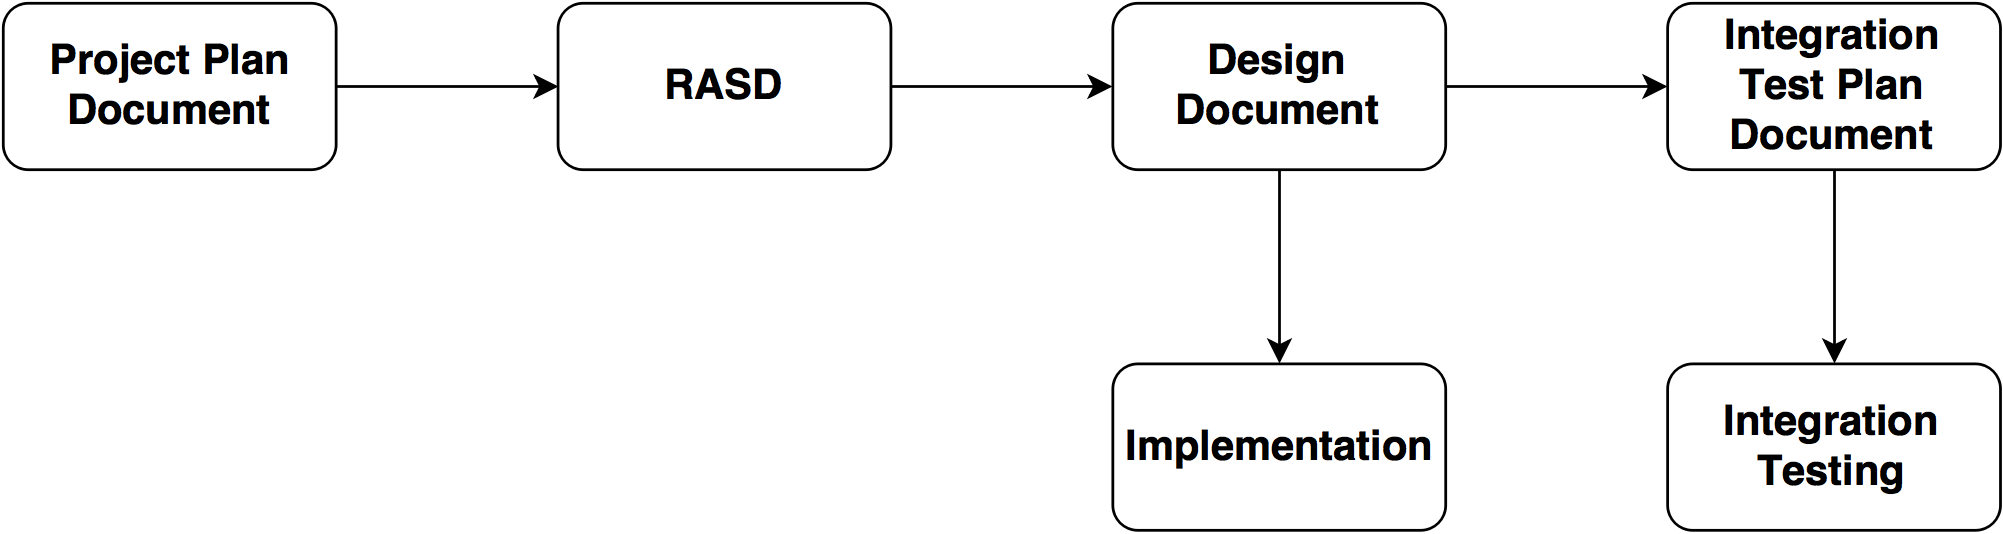
\includegraphics[width=\textwidth]{./pictures/dependencies_dag.png}}
		\caption{Dependency graph illustrating precedence constraints.}
		\label{dep_dag}
\end{center}
\end{figure}
\noindent
The following is a Gantt chart to describe the chosen schedule for the project:

%gantt chart here

\section{Resource Allocation}

\chapter{Risk Management} \label{risk_man}
%Risk management
%Problemi di interazione con il payment handler e il maintenance system

The \emph{PowerEnJoy} system project might be threatened by many risks. The analysis of said risks follows a specific approach that splits them up into three groups: \textit{project}, \textit{technical} and \textit{business risks}.

\section{Project Risks}
\textit{Project risks} pose a threat to the project plan and make the project schedule slip, increasing the overall costs.
The following risks have been found and analysed, providing a response strategy. 
\begin{description}
\item[Changes concerning requirements:] during the development of the project the requirements can change unexpectedly. This kind of risk cannot be prevented, but it can be reduced by using a style of programming that takes advantage of reusable and extensible code.
\item[Deadlines are not met:] it can occur that the project requires more time than expected to be carried out. In this case only some functionalities will be offered in a first release while less essential features will be developed later. The above-mentioned first release can provide the target services by the only means of the Mobile Application. The Web Application and the Web Tier may be built afterwards.
\item[Lack of communication:] team members usually work separately. This can cause misunderstandings and conflicts about the division of different tasks. To mitigate the risk, crystal clear and complete specification and design documents must be provided. Moreover the responsibilities of each group member must be clearly defined in this document.
\item[Team break-ups:] if, for any natural or human reason, any of the team member is forced to leave the project team, the development process will inevitably suffer from huge delays and the risk will result in an impossibility to meet the defined deadlines (this is due to the very small size of the team). This can be countered, in case of social issues, in a pre-emptive way by implying a work method that values each team member in the same way; in case of natural causes, the reactive behaviour to be adopted must be that of hiring new members. Note that, in this second unpredictable case, the time required by the project will be greatly increased also due to the well-acknowledged Brooks's Law~\cite{mythical-man-month}.
\end{description}

%tabella con catalogazione rischi

\section{Technical Risks}
\textit{Technical risks} threaten the quality and the punctuality of the software product preventing a straightforward implementation.
The following risks have been found and analysed, providing a response strategy. 
\begin{description}
\item[Unreadable code:] large projects may have a badly structured and unreadable code. Documenting the code can be a reasonable way to mitigate this risk. Furthermore, information provided by a good Design Document can come in handy too.
\item[Scalability issues:] if the system does not scale properly with the increasing number of users, a work of major redesign will be carried out. To reduce the risk, a correct estimation of the computing power and the number of involved machines is necessary.
\item[Integration testing failure:] in case, during the integration testing phase, the team realizes that the system components do not integrate as they should based on the tests defined in the ITPD~\cite{itpd}, there can be the risk of delays in the overall project schedule, resulting in a fail in meeting deadlines. In case this happens, the efforts of the team members will be fully redirected to redefining and implementing integration test cases over other tasks in progress.
\item[Downtime:] Upon being fully functional and operative, the system may experience brief or long periods of downtime. This will be accounted for and discussed in other documents, and the risk could be made less likely by decoupling the clients' activities and making some clients independent from other components of the system, so that a channel to access the application is always active while the other is being fixed. In cases in which this is not possible, structuring the code to make it more reliable, robust and maintainable is always a good countermeasure.
\item[Data loss and leaks:] if, for any reason, a big portion of the application data should be lost, the damage to the application itself could be considerable. For this reason, it is recommendable to store data in multiple locations, or to have one or more backup database, especially for sensitive information.
\end{description}

%tabella con catalogazione rischi

\section{Economical Risks}
\textit{Economical risks} jeopardize the whole software product threatening its viability.
The following risks have been found and analysed, providing a response strategy. 
\begin{description}
\item[Bankruptcy:] the income from the usage of the application may not be sufficient to support maintenance and development of the system. A good feasibility study should help avoiding this critical situation.
\item[Local regulation and policies:] minor risks could derive from changes in the local regulation about traffic within the city, and especially with respect to the areas that will be covered by the service. The minor problems deriving from this can be mitigated by maintaining a continuous dialogue with the local administration for the city (potentially, cities) in which the \textit{PowerEnJoy} service will be deployed.
\item[Competitors:] competition by other providers of the same kind of services must be kept in consideration at all times, since a poor management could lead considerable economical losses. Competition must be exploited to the advantage of the \textit{PowerEnJoy} company by continuously providing new appealing functionalities, based in part on customer feedback.
\end{description}

%tabella con catalogazione rischi

\appendix
\chapter{Appendix}
\section{Software and tools used}
\begin{itemize}
\item \LaTeX, used as typesetting system to build this document.
\item draw.io - \url{https://www.draw.io} - used to draw diagrams and mock-ups.
\item GitHub - \url{https://github.com} - used to manage the different versions of the document and to make the distributed work much easier.
\item GitHub Desktop, the GitHub official application that offers a seamless way to contribute to projects.
\end{itemize}
\section{Hours of work}
The absolute major part of the document was produced in group work. The approximate number of hours of work for each member of the group is the following:

\begin{itemize}
\item Giovanni Scotti: 25 hours
\item Marco Trabucchi: 20 hours
\end{itemize}

NOTE: indicated hours include the time spent in group work.

\begin{thebibliography}{1}

\bibitem{ieee-29148}
	ISO/IEC/IEEE 29148:2011 \emph{Systems and software engineering - Life cycle processes - Requirements engineering}
	
\bibitem{se-assignments}
	AA 2016/2017 Software Engineering 2 - \emph{Project goal, schedule and rules}

\end{thebibliography}

\end{document}